\documentclass{article}


\usepackage[left=3cm,right=3cm,top=3.5cm,bottom=4cm]{geometry}

\usepackage{ucs}
\usepackage[ngerman]{babel}
\usepackage[utf8x]{inputenc}
\usepackage[T1]{fontenc}
\usepackage{siunitx}
\usepackage{listings}
\usepackage{setspace}
\usepackage{lmodern}
\usepackage{graphicx}
\usepackage{xcolor}
\definecolor{forestgreen}{RGB}{34,139,34}
\usepackage{subcaption}
\captionsetup[subcaption]{list=true}

\usepackage[backend=bibtex,sorting=none]{biblatex}
\addbibresource{main.bib}

\begin{document}

\begin{titlepage}
        \begin{center}
                {\scshape\LARGE Hochschule Bremen \par}
                \vspace{1cm}
                {\scshape\Large Fakultät 4 \par}
                \vspace{1cm}
                {\Large\itshape Schienennetz der Deutschenbahn in Openlayer mit Blick auf Schadstoffausstoß\par}
                \vspace{1cm}
                {\rmfamily\large  Geodatenverarbeitung \par}
                {\rmfamily\large  Dr.-Ing. Christian Seip\par}
                \vspace{2cm}
                {\large
                        \begin{tabular}{ll}
                        Jannick Bock & 5124529\\
                \end{tabular}
                }
        \end{center}
        \vfill
\end{titlepage}

\pagebreak
\tableofcontents
\pagebreak
\section{Einleitung}
Die Schadstoffemissionen sind in den letzten Jahren in Deutschland angestiegen, deshalb gibt es mittlerweile auch Dieselfahrverbote in einigen Städten Deutschlands.\cite{nox}
Auch der Schienenverkehr ist an dem Anstieg der Emission nicht ganz unbeteiligt. Durch die nicht flächendeckende Elektrifizierung des Streckennetztes stößt auch die Deutsche Bahn mit dieselbetriebenen Person und -Güterverkehr reichlich Stickoxide auch NOX genannt in die Luft. Auch der CO2 Ausstoß sämtlicher Antriebe der Deutschen Bahn ist beachtlich. Anhand des Opendata Portals der Deutschen Bahn \cite{dbgeodaten} können Daten zum Streckennetz und zur Umweltbelastung entnommen werden.

\subsection{Zielstellung}
Die folgende Arbeit soll das Deutsche Schienennetz aus dem opendata Bereich der Deutsche Bahn visualisieren. Zudem soll das Schienennetz in anbetracht der Schadstoffemissionen des Zugverkehrs aufzeigen an welchen Orten in Deutschland  hohe Emmisionsbelastung im Jahr 2014 entstanden sind. Es gilt aufzuarbeiten welche Gründe ein erhöhter Emissionswert also Stickoxid oder CO2 Ausstoß an einer bestimmten Stelle in Deutschland hat. Dies kann eine nicht elektrifizerte Streckenabschnitt oder eine erhöhte Belastung zum Beispiel in Dichtbesiedelten Gebieten sein. Diese Fragestellung soll durch eine Visualisierung des Streckennetz und der Emissionen beantwortet werden.
\\\\
Zusätzlich wird das Schienennetz auf Geschwindigkeit untersucht, also es gilt auszuarbeiten, welche Abschnitte für zum Beispiel den ICE 3 mit einer Höchstgeschwindigkeit von 300 km/h ausgerichtet sind.\cite{ice3}
\subsection{Architektur }
Die Architektur ist sehr simpel gehalten. Es gibt einen Geoserver der in seinem Datenverzeichnis zugriff auf die Shape-Files und die dazugehörigen Attribute hat.
Als Frontend wird Javascript mit der Openlayer-Bibliothek verwendent.\cite{openlayer}

\pagebreak
\section{Datenbeschaffung}



\subsection{Beschreibung der Daten}
\subsubsection{Streckennetz}

Woher die Daten, welchem Format, Stand
Beschreibung
\subsubsection{Schadstoffdaten}

\subsection{Aufbereitung der Daten}

\pagebreak
\section{Aufsetzen eines Geoservers}


\subsection{Einrichtung}
\subsection{Styling}

\pagebreak
\section{Webapp mit Openlayer}

Die Webapplikation wurde in HTML und Javascript programmiert. 
Als Dependencymanagementsystem wurde NPM benutzt.
Für das Deployment wurde der Webapplikations Bundler Parcel genutzt. Dieser Budnler deployed die Webapplikation standartmäßig auf Localhost mit dem Port 1234.


Für dieses Projekt wurde die Openlayer Version 6.3.1 verwendet.
Auf der HTML Seite ist eine Map und ein Title integriert.
Darunter sind alle Legenden der Layer als einzelne Bilder dargestellt.


Als Kartenhintergrund wurde Openstreetmap gewählt. Dies soll die Visualisierung der Streckenabschnitte unterstützen, um zum Beispiel zu erkennen welcher lokale Abschnitt nicht als elektrifiziert gekennzeichnet ist.
Zusätzlich wurde das aktuelle online verfügbare Openrailwaymap als Layer verfügbar gemacht.

Darüber werden dann die Layer gelegt die den Schadstoffausstoß visualisieren.
Die Oberste Schicht bilden dann die Layer die das Streckennetzabbilden.

Um eine erste übersichtliche Darstellung zu ermöglichen sind nur die Layer von Openstreetmap und der Bahnnutzunglayer aktiviert.
Die erste vordefinierte View ist auf Deutschland zentriert.
Die initialisierte Map sieht wie folgt aus.

\begin{lstlisting}[frame=single,basicstyle=\small]
const map = new Map({
        target: 'map',
        layers: [osm,openrailwaymap,
	co2Rail,noxKGRail,
	basicNutzung,elektrNutzung,geschNutzung],
        view: view
});
\end{lstlisting}


Alle Layer sind über den integrierten LayerSwitcher aus/einschaltbar.
Der LayerSwitcher ist eine Community Erweiterung für Openlayer. \cite{layerswitcher}. Er ist als MapControl Objekt zur Map hinzuzufügen.
\begin{lstlisting}[frame=single,basicstyle=\small]
var layerSwitcher = new LayerSwitcher({
        tipLabel: 'Legende',
        groupSelectStyle: 'none' 
});

layerSwitcher.useLegendGraphics = true;
map.addControl(layerSwitcher);
\end{lstlisting}


\subsection{WMS Service}

Um die Layer in diese Webapplikations zu integrieren wird der WebMapServer vom Geoserver angesprochen.
Dafür wird das TileWMS Objekt genutzt.
\begin{lstlisting}[frame=single,basicstyle=\small]
var wmsSource = new TileWMS({
        url: 'http://localhost:8080/geoserver/wms',
        params:{'LAYERS': 'DeutscheBahn:Bahnnutzung','TILED': true},
        serverType: 'geoserver',
        crossOrigin: 'anonymous'
});
\end{lstlisting}
Es wird auf die URL des WMS Service zugegriffen mit dem entsprechenden Layer den man laden möchte.
Es wurde sich entschieden alle Layer als 'Tiled' Layer anzuzeigen, so ist es möglich nur die relevanten Layerinformationen zu laden, um performance zu sparen.

Um nun aus dem TileWMS einen layer zu machen, wird ein neues TileLayer Objekt erzeugt.

\begin{lstlisting}[frame=single,basicstyle=\small]
var basicNutzung = new TileLayer({
        title: 'Bahnnutzungsarten (DB-Daten 2019)',
        source: wmsSource,
        minZoom: 5
});
\end{lstlisting}

Es wurde für alle Layer ein Titel deklariert, der so in den LayerSwitcher übernommen wird. Eine mindest Zoom Stufe wurde angegeben, um den Layer nur anzuzeigen wenn man auch nah genug auf ihn gezoomt hat, um performance zu sparen.

Auf diese Weise wurden alle Layer mit Polygonlinien eingebunden.
Die Layer für die Schadstoffemissionen CO2 und NOX wurden zusätzlich noch mit einem Opacity wert von 0.6 parametrisiert, um nicht den Openstreetmap layer komplett zu überlagern. 

\subsection{Legende Anzeige}
Um dem Nutzer ständig zu informieren, welche Farbe eines Layers welche Information bedeutet, werden die Legenden aus den Layer-Styles generiert.

Dazu werden alle erstellten TileWMS in ein Array hinzugefügt und dann wird beim Laden der Seite, auf die LegendUrl der einen Quellen zugegriffen. Diese liefern Bilder der Legendenbeschreibung zurück. Die erhaltenen Bilder werden in ein HTML-div Element angehängt.


\begin{lstlisting}[frame=single,basicstyle=\small]
function createLegends(){
var resolution = map.getView().getResolution();
         sourceList.forEach(a => {
                
                var x = document.createElement("IMG");
                x.src = a.getLegendUrl(resolution);
                
                 var layer = JSON.stringify(a.getParams());
                 x.title= JSON.stringify(a.getParams());
                 x.alt= JSON.stringify(a.getParams());
                 document.getElementById("legends").appendChild(x);
        });
}
\end{lstlisting}


\pagebreak
\section{Ergebnisse}

\subsection{Webansicht}

Die Standardansicht der Webseite sieht wie folgt aus. 
\begin{figure}[h]
\centering
	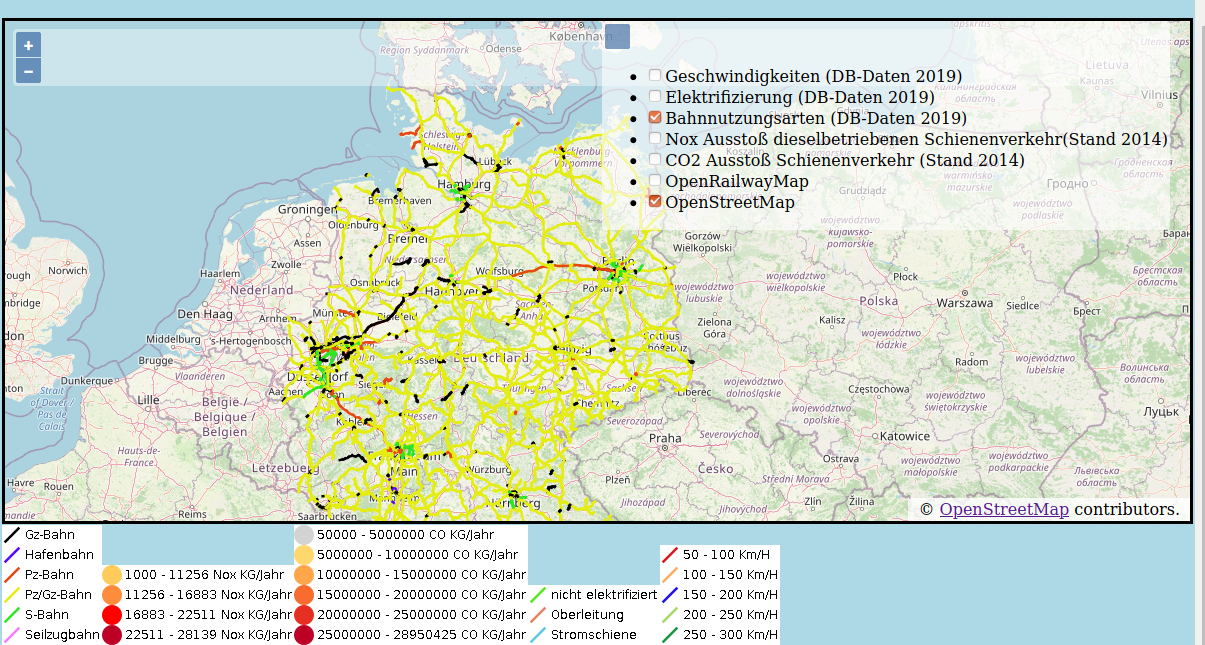
\includegraphics[width=0.9\textwidth]{images/defaultview.png}
	\caption{Default view from the webapplikation}
\end{figure}
Zentral wird die Karte mit der aktuell ausgewählten Zoomstufe angezeigt. Die Zoomstufe lässt sich über die Buttons oben links ändern. Auf der rechten Seite ist der LayerSwitcher zu sehen, dieser ermöglicht es alle Layer in verschiedenen Kombinationen anzuzeigen. Am Unteren Rand der Karte sind die Legenden der Layer zu erkennen.
\pagebreak
\subsection{Datenanalyse}
Anhand der Visualisierung sind einige Auffälligkeiten zu erkennen.

In Norddeutschland auf der Zugstrecke auf die Insel Sylt gibt es einen der höchsten Ausstoß von Stickoxide durch den Dieselverkehr in Deutschland. In Norddeutschland sind ungefähr ein drittel der Bahninfrastruktur elektrifiziert.\cite{marschbahn} Und da regelmäßig Dieselloks auf die Insel Sylt fahren um den Tourismus zu unterstützen, ist dies eine vielbefahrene Strecke. Diese Strecke führt über den Hindenburgdamm eingleisig nach Sylt, dies bedeutet es kann auch häufig zum Stau kommen, welcher ebenfalls für die erhöhte Umweltbelastung spricht. \cite{marschbahn}
\begin{figure}[h]
\centering
	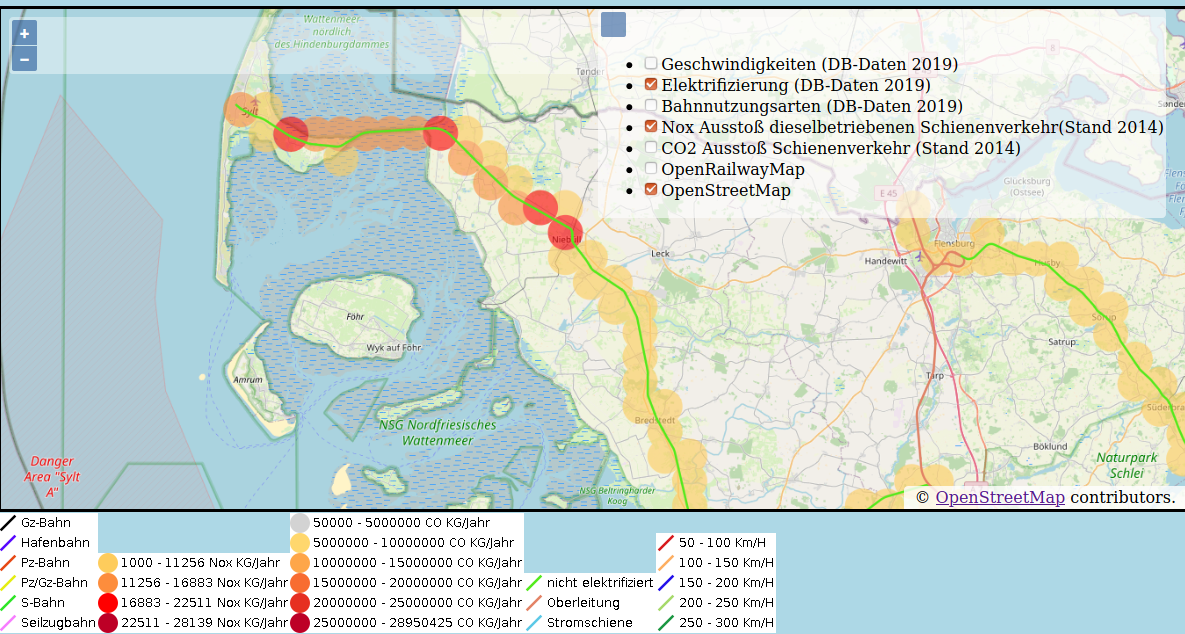
\includegraphics[width=0.7\textwidth]{images/Analyse1.png}
	\caption{Stickoxid Ausstoß in Norddeutschland}
\end{figure}

Der Ausstoß von CO2 ist nur den Ballungsgebieten deutlich erhöht. Die höchsten gemesenen Werte Gemessener Ausstoß vom Schienenverkehr in dichtbesiedelten Städten höher.
\begin{figure}[h]
\centering
	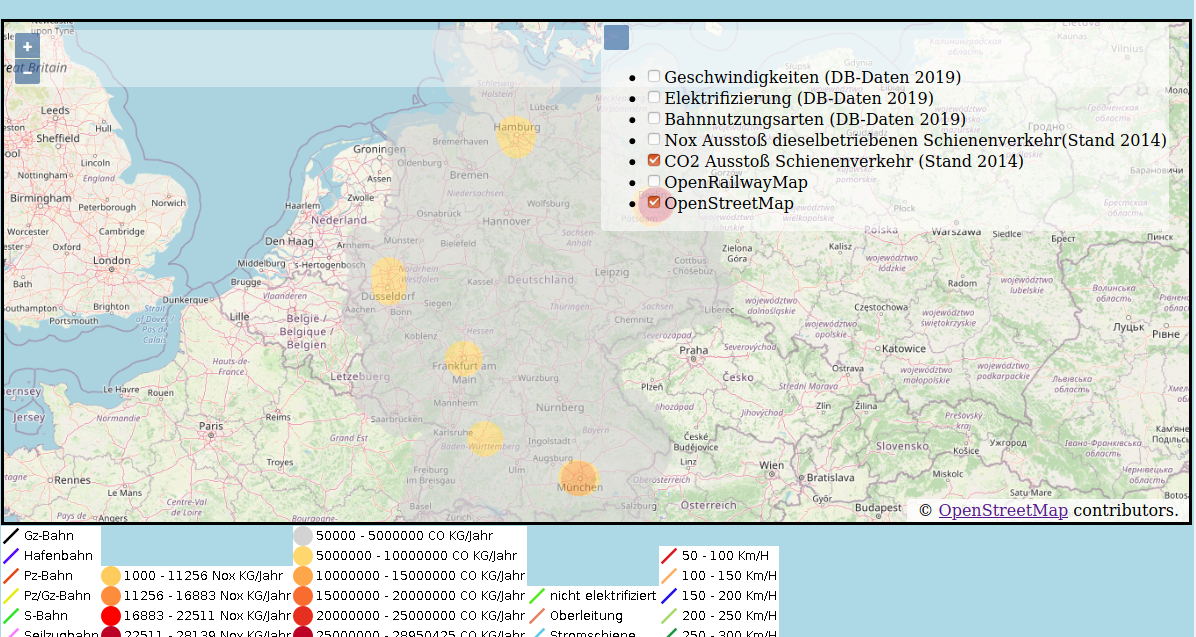
\includegraphics[width=0.7\textwidth]{images/Analyse3.png}
	\caption{CO2 Ausstoß der Deutschen Bahn}
\end{figure}


Ein weiterer Aspekt der im aktuellen Deutschenschienennetz auffällt, ist das sehr wenig Strecken auf Höchstgeschwindigkeit ausgelegt sind. Was bedeutet, dass ICE vorallem der neueren Generationen nur auf kurzen Streckenabschnitten die Gelegenheit haben ihre maximal Geschwindigkeit zu erreichen.

\begin{figure}[h]
\centering
	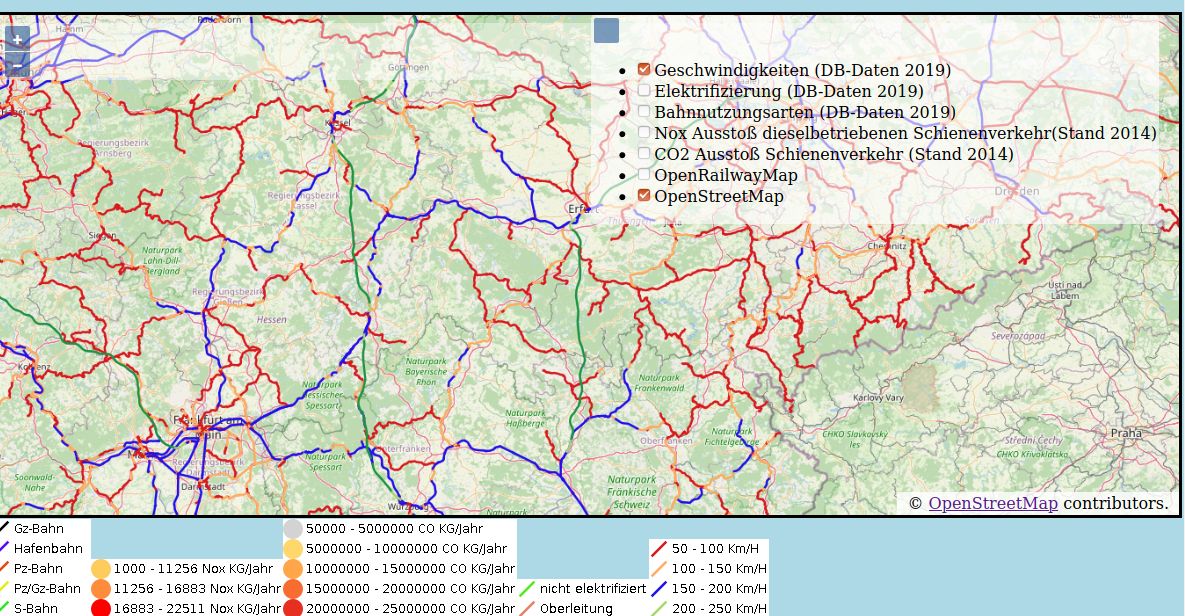
\includegraphics[width=0.7\textwidth]{images/Analyse2.png}
	\caption{Ausschnitt der Höchstgeschwindigkeit des Streckennetztes}
\end{figure}

Die Strecken ab Mitteldeutschland bis Süddeutschland sind teilweise auf bis zu 300 Km/h ausgerichtet. Von Westdeutschland nach Ostdeutschland gibt es keine Einzige Strecke die für Höchstgeschwindigkeit eines ICE ausgerichtet ist.
Die meisten Streckenabschnitte in Deutschland bieten eine Höchstgeschwindigkeit von 150 - 200 Km/h.

\pagebreak
\section{Installationsanleitung}
Dies ist eine Installationsanleitung für Ubuntu 18.04.
\subsection{Git Verzeichnis clonen oder ZIP Download}
Das Git Projekt clonen oder als Zip-Downloaden.
Über Github kann das Projekt als ZIP oder über Git clone heruntergeladen werden.

Im Repository ist der geoserver und die geoinfoweb Verzeichnise. 

\subsection{Pfade setzen}
Den JAVAHOME Pfad zu der installieren Java Umgebung setzen.
Den GEOSERVERHOME Pfad zu dem beigefügtem Geoserver setzen.

Als Ubuntu-Beispiel (Pfade können abweichen) :
\begin{lstlisting}[frame=single,basicstyle=\small]
echo "export GEOSERVER_HOME=entpackterPfad/geoinfo/geoserver" >>/etc/environment
echo "JAVA_HOME=/usr/lib/jvm/java-11-openjdk-amd64" >>/etc/environment
\end{lstlisting}


\subsection{Start GeoServer und Frontend}
Sind die beiden Home Pfade gesetzt kann man in den ../geoserver/bin Ordner wechseln und die startup.sh ausführen.


Nun sollte der Geoserver auf localhost:8080 erreichbar sein.
Der Login kann über den Standard User : admin
PW: geoserver erfolgen.


Um das Frontend zum laufen zu bekommen muss man in den "geoinfoweb" Ordner des Repository wechseln.
 NPM muss für die folgenden Schritte installiert sein
Dann führt man die folgenden Befehle aus.
\begin{lstlisting}[frame=single,basicstyle=\small]
1. npm init
2. npm start
\end{lstlisting}
 "Npm start" kompiliert das Frontend und deployed es auf "http://localhost:1234/"
 

\pagebreak
\addcontentsline{toc}{section}{Abbildungsverzeichnis}
\listoffigures
\pagebreak
\printbibliography
\end{document}
